% Compile with pdflatex

\documentclass[a4paper,10pt]{article}

\usepackage[utf8]{inputenc}
\usepackage{pgfplots}
\usepackage{tikz}
\usepackage{array,tabularx}
\usepackage{amsmath}

\newenvironment{conditions*}
  {\par\vspace{\abovedisplayskip}\noindent
   \tabularx{\columnwidth}{>{$}l<{$} @{\ : } >{\raggedright\arraybackslash}X}}
  {\endtabularx\par\vspace{\belowdisplayskip}}


\newcommand{\laplace}{\mathcal{L}}
% \pgfplotsset{width=7cm,compat=1.8}

% Title Page
\title{The Logarithmic Filter}
\author{José M. González}


\begin{document}
\maketitle

\begin{abstract}
This document gathers technical information for building a logarithmic filter.
\end{abstract}

\section{Goal}

In the aim of making a linear filter for the ear we have to take into account the
logarithmic sensibility of the cochlea to the frequencies. 

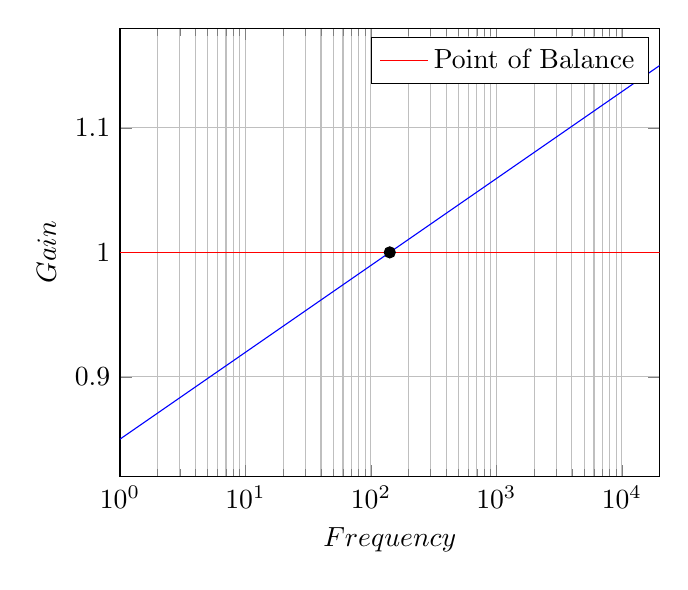
\begin{tikzpicture}
  \begin{semilogxaxis}[
    xmin=1, xmax=2e4, domain=1:20000,
    grid=both,
    xlabel=$Frequency$,
    ylabel=$Gain$
  ]

    \addplot[red] {1};
    \addlegendentry{Point of Balance} 

    \addplot[blue] {0.030292359 * ln(x) + 0.85 };
   
    \addplot[black, mark=*] 
            plot[errors bars/.cd]
            coordinates {(141.421356237,1)};
    
  
  \end{semilogxaxis}
\end{tikzpicture}

$Gain=1$ Point of Balance

\section{Equations}

\begin{equation}
 G(f) = m \log_s{f} + G_0 - m \log_s{F_{MIN}}
\end{equation}
 
where

\begin{conditions*}

G & Gain \\
G_0 & Initial Gain or $G(F_{MIN}) = 1 - \delta$ \\
s & Scale \\
f & Frequency \\
F_{MIN} & Lower frequency \\
F_{MAX} & Upper frequency \\
B & Point of Balance \\
m & slope 
 
\end{conditions*}

Or taking $C$ as $C= G_0 - m \log_s{F_{MIN}} $ 

$$ G(f) = m \log_s{f} + C $$

or even expressed as the natural logarithm,

$$G = m \frac{\ln{f}}{\ln{s}} + C $$

If $G$ is defined as $1 \pm \delta $ we get, some useful equations.

\begin{eqnarray} 
  2 \delta & = & m \log_s { \frac{F_{MAX}}{ F_{MIN} } } \\
  m & = & \frac{2 \delta }{ \log_s{ \frac{F_{MAX}}{F_{MIN}} }} \\
  \ln{B} & = & \frac{1}{2} \log_s{ F_{MAX} \cdot F_{MIN}} \\
      B  & = & \sqrt{F_{MAX} \cdot F_{MIN}}  
\end{eqnarray}

$m$ and $s$ work in pair, $ s = s(m) $.

$$ \ln{s} = \frac{2 \delta}{ m \ln{ \frac{F_{MAX}}{F_{MIN}}} }  $$


A non logarithmic representation:


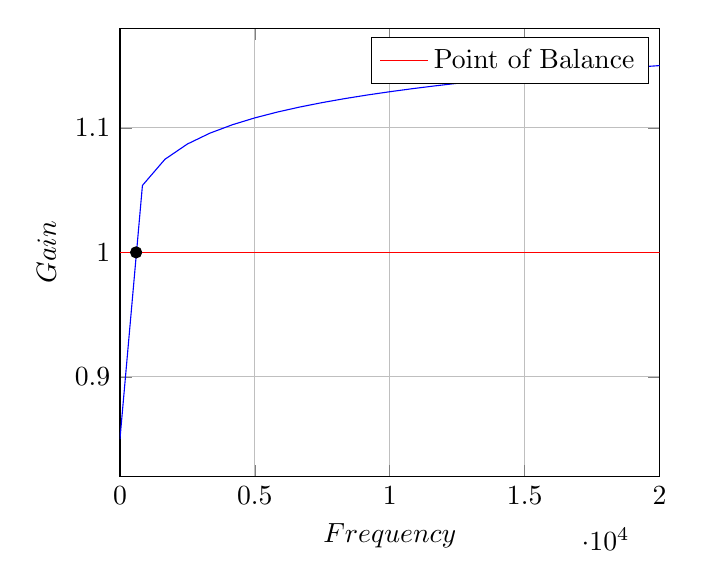
\begin{tikzpicture}
  \begin{axis}[
    xmin=1, xmax=2e4, domain=1:20000,
    grid=both,
    xlabel=$Frequency$,
    ylabel=$Gain$
  ]

    \addplot[red] {1};
    \addlegendentry{Point of Balance} 

    \addplot[blue] {0.030292359 * ln(x) + 0.85 };
   
    \addplot[black, mark=*] 
            plot[errors bars/.cd]
            coordinates {(600, 1)};
    
  \end{axis}
\end{tikzpicture}

\section{Transfer Function}

Let's suppose,

\begin{equation}
 H(j\omega) = m \ln{j\omega} + 1 - \delta - m \ln{F_{MIN}}
\end{equation}

or just

\begin{equation}
 H(j\omega) = m \ln{j\omega} + C
\end{equation}

and let's us assume

$$ s = j\omega $$
$$ H(s) = m \ln{s} + C $$

The Inverse Laplace transformation $h(t) = \laplace^{-1} \lbrace F(s) \rbrace $ can be obtained
by knowing:

\begin{eqnarray}
\laplace \lbrace \alpha f(t) + \beta g(t) \rbrace & = & \alpha F(s) + \beta G(s) \\
\laplace \lbrace -t \cdot f(t) \rbrace & = & \frac{d}{ds} F(s) \\
\laplace \lbrace \delta(t) \rbrace & = & 1 \\
\laplace \lbrace u(t) \rbrace & = & \frac{1}{s} 
\end{eqnarray}

So,

$$ \laplace^{-1} \lbrace m \ln{s} + C \rbrace = \laplace^{-1} \lbrace m \ln{s} \rbrace + C \cdot \delta(t) $$

and

\begin{eqnarray}
 t \cdot h(t) & = & \laplace^{-1} \lbrace \frac{d}{ds} (m \ln{s}) \rbrace \\
              & = & m \cdot \laplace^{-1} \lbrace \frac{1}{s}) \rbrace \\
              & = & m \cdot u(t)
\end{eqnarray}

all together,

\begin{equation}
  \boxed{ h(t) =  \frac{m \cdot u(t)}{t} + C \cdot \delta(t) }
\end{equation}

\section{Approach}

So we suggest to try the convolution

$$ y(t) = h(t) \ast x(t) $$

in a discretized way.


\end{document}          



Impulse response